The dataset to perform the analysis should include, at the most granular level possible, the share of votes received by the candidate ($\overline{Y}_g$), a partition of the voting population in categories of interest (e.g, ethnic categories, which represent $\overline{X}_g$) and covariates at that same geographical level ($Z_g$).

The most granular level for electoral results in the United States is the electoral precinct, whose dimension is typically in the order of hundreds of a couple of thousands of voters.

Census data, instead, are collected at different geographical levels, with geographical levels varying with the variables of interest.

The most granular level for census data is the census block, which is a geographical unit that is typically bounded by geographical features either natural (e.g., rivers) or artificial (e.g., streets). Given their geographical definition, census blocks are quite different in population size, with a considerable amount of blocks being uninhabited, and the most populated ones (typically in urban areas) having a population of hundreds of people.

The only variables collected at the census block level are the total population, the voting age population, ethnic composition and the number of housing units. Moreover, these variables are collected at the census block level only in the decennial census, which is conducted every ten years.

Census blocks are then grouped into larger geographical units, which are used to collect other variables of interest. In particular, the census block groups (CBGs) are the smallest geographical unit for which the American Community Survey (ACS) collects data on a yearly basis. CBGs are typically composed of a few hundred to a few thousand people, and they are designed to be relatively homogeneous in terms of population characteristics.

Variables collected at the CBG level in ACS include several socio-economic characteristics, such as income, educational attainment, employment status, as well as language spoken at home, commuting patterns, and housing characteristics. The ACS data are collected through sample surveys, so that data at the CBG level are subject to sampling variability.

Finally, census block groups are grouped into larger geographical units, which are called census tracts.

The electoral precincts, instead, are geographical units that are defined by the electoral authorities for the purpose of organizing elections. Precincts are typically composed of a few hundred to a few thousand voters, and they are sometimes denoted as voting districts (VTDs).

VTDs, however, are not units of the census, and they are not completely aligned with CBGs. VTDs are always constituted by a set of census blocks, and they are contained within a single census tract, but they can cross the boundaries of CBGs. This means that a VTD can contain parts of multiple CBGs, and a CBG can be split across multiple VTDs; viceversa is also true.

Fig. \ref{fig:census-geographical-units} shows a schematic representation of a possible relationship between census blocks, CBGs, census tracts and VTDs.

\begin{figure}[htbp]
	\centering
	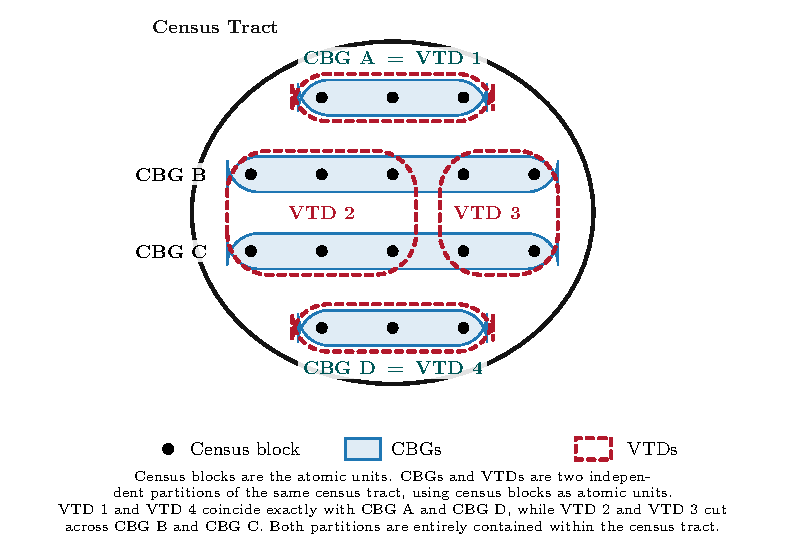
\includegraphics[width=\textwidth]{Images/Census_sets/census_sets_v2.pdf}
	\caption{Relationship between electoral precincts (VTDs), census blocks, census block groups (CBGs), and census tracts.}
	\label{fig:census-geographical-units}
\end{figure}

Some of the variables of possible interest for the analysis are collected only at the CBG level in ACS surveys. Therefore, a procedure to aggregate the data at the VTD level was necessary.

ALARM dataset by \citet{t._kenny2021} combine electoral results at the VTD level previously collected by \citet{vest2020precinct} with demographic data of 2020 US census collected by \citet{uscensus2020}.

That provides a dataset that includes the share of votes received by the candidates at the VTD level, as well as the total population and the voting age population at the census block level with the corresponding ethnic composition.

This dataset, while being very useful, does not include the socio-economic characteristics, which are of fundamental importance for the analysis, and which are collected at the CBG level in ACS surveys.
ACS data are easily accessible through the \texttt{tidycensus} package in R \citep{tidycensus}.

The following passage involved exploiting \citet{census2021baf}'s files, which provide the mapping of census blocks to CBGs and VTDs, to aggregate the socio-economic characteristics collected at the CBG level in ACS surveys to the VTD level.

As in Fig. \ref{fig:census-geographical-units}, we can think of three scenarios: VTDs that perfectly align with one CBG, VTDs that aling with exactly two or more CBGs, and VTDs that cross the boundaries of CBGs.

For the first scenario, the aggregation of socio-economic characteristics from CBGs to VTDs is straightforward: the characteristics of the VTD are simply the same as those of the corresponding CBG.

The second scenario is also straightforward: the socio-economic characteristics of the VTD are simply the either the sum (in case of counts, e.g, population or the number of people with a college degree) or the average (in case of other quantities, e.g. median income) of the socio-economic characteristics of the CBGs that compose it.

The third scenario is a bit more complicated and required a procedure to apportion the socio-economic characteristics of the CBGs that are crossed by the VTD boundaries.

The procedure rested on the assumption that that differences in the apportionment of census blocks in the construction of the VTDs and CBGs are independent of the socio-economic characteristics of the population.

That assumption is partly disputable, because the electoral authorities in the United States have been known to engage in gerrymandering, which is the practice of drawing electoral district boundaries in a way that favors a particular political party or group.
However, gerrymandering is typically done at the level of congressional districts, without particular interventions at the level of VTDs.

Moreover, census block groups are designed to be relatively homogeneous in terms of population characteristics, so that the differences in apportionment of census blocks between VTDs and CBGs are likely to be small.

Therefore, I have assumed that the average socio-economic characteristics of the population in a CBG are the same as those of the population in the census blocks that compose it.
Subsequently, I have constructed fictitious populations of the census blocks, assigning to each census block the average socio-economic characteristics of the population in the corresponding CBG.

I will give two examples of the procedure, one for a count variable and one for a non-count variable: if a CBG with population of 1000 people has 200 people with a college degree, I have assumed that each census block in that CBG has 20\% of its population with a college degree, so that a census block with 100 people has 20 people with a college degree; on the other side, if a CBG has a income of \$50,000, I have assumed that each census block in that CBG has a median income of \$50,000.

Finally, I have aggregated the fictitious populations of the census blocks to the VTD level, obtaining an estimate of the socio-economic characteristics of the population in each VTD.
Obviously, these estimates are subject to some error, partly arising from the sampling errors in the original ACS data, and partly from the apportionment procedure.


However, this procedure is easily implementable and can be applied to any variable of interest that is collected at the CBG level.

%Electoral data at precinct level for 2020 US elections have been collected and made available by \citet{vest2020precinct}.